\chapter{HASIL DAN UJI COBA}
Pada bab ini akan dipaparkan hasil uji coba saat sistem dijalankan. Uji coba sistem TPORT akan dilakukan untuk memastikan kualitas perangkat lunak yang dikembangkan dengan analisis dan perancangan perangkat lunak.
\section{Lingkungan Uji Coba}
Lingkungan uji coba sistem pada Kerja Praktik kali ini meliputi perangkat keras dan perangkat lunak adalah sebagai berikut:
\begin{enumerate}
	\item Perangkat Keras
	\begin{itemize}
		\item \textit{Processor} Intel® Core™ i7-5500U CPU @ 2.40GHz
		\item Memori 4 GB
	\end{itemize}
	\item Perangkat Lunak
	\begin{itemize}
		\item Sistem Operasi Ubuntu 16.04 LTS 64 bit.
	\end{itemize}
\end{enumerate}

\section{Skenario Pengujian}
Skenario pengujian yang akan dilakukan pada aplikasi TPORT adalah melakukan peran sebagai admin yang sedang membuka aplikasi. Langkah-langkah dari skenario adalah sebagai berikut:
	\begin{enumerate}
	\item Pengguna membuka aplikasi TPORT
	\item Pengguna memilih menu \textit{upload}, \textit{request}, dan target
	\item Pengguna menambahkan data pencapaian \textit{revenue} dengan mengupload file pada halaman upload
	\item Pengguna melihat detail hasil pencapaian \textit{revenue} pada halaman \textit{request}
	\end{enumerate}
	
\subsection{Pengujian Mengupload Data Pencapaian \textit{Revenue}}
Pengujian ini dilakukan terhadap fungsionalitas \textit{upload} data pencapaian \textit{revenue}. Tabel \ref{tab:list_upload} menjelaskan pengujian fungsionalitas ini.

\begin{table}[h!]
	\centering
	\begin{tabular}{|p{4cm}|p{6cm}|}
	\hline
	Kode \textit{Use Case} & UC-001\\ \hline
	Tujuan Pengujian & \textit{Upload} semua data hasil pencapaian \textit{revenue}\\ \hline
	Data Masukan & File .csv \\ \hline
	Prosedur Pengujian & 
		\begin{enumerate}
		\item Pengguna \textit{login} sebagai administrator
		\item Pengguna memilih menu \textit{upload}
		\end{enumerate}\\ \hline
	Hasil yang diharapkan & Semua data hasil pencapaian \textit{revenue} dapat di-\textit{upload} dan data yang di-\textit{upload} dapat masuk ke basis data sistem \\ \hline
	Hasil yang diperoleh & Semua data hasil pencapaian \textit{revenue} dapat di-\textit{upload} dan masuk ke basis data sistem \\ \hline
	Kesimpulan & Proses \textit{upload} hasil pencapaian \textit{revenue} berhasil \\ \hline
	Kondisi Akhir & Data hasil pencapaian \textit{revenue} masuk ke basis data sistem\\ \hline
	\end{tabular}\caption{Skenario Pengujian \textit{Upload} Data Hasil Pencapaian \textit{Revenue}}
	\label{tab:list_upload}
\end{table}

\subsection{Pengujian Mengelola Target Pencapaian \textit{Revenue}}
Pengujian ini dilakukan terhadap fungsionalitas mengelola target pencapaian \textit{revenue}. Tabel \ref{tab:list_target} menjelaskan pengujian fungsionalitas ini. Gambar \ref{figure:lihatTarget} adalah hasil fungsionalitas menampilkan target serta mengubah target.

\begin{figure}[h!]
\centerline
{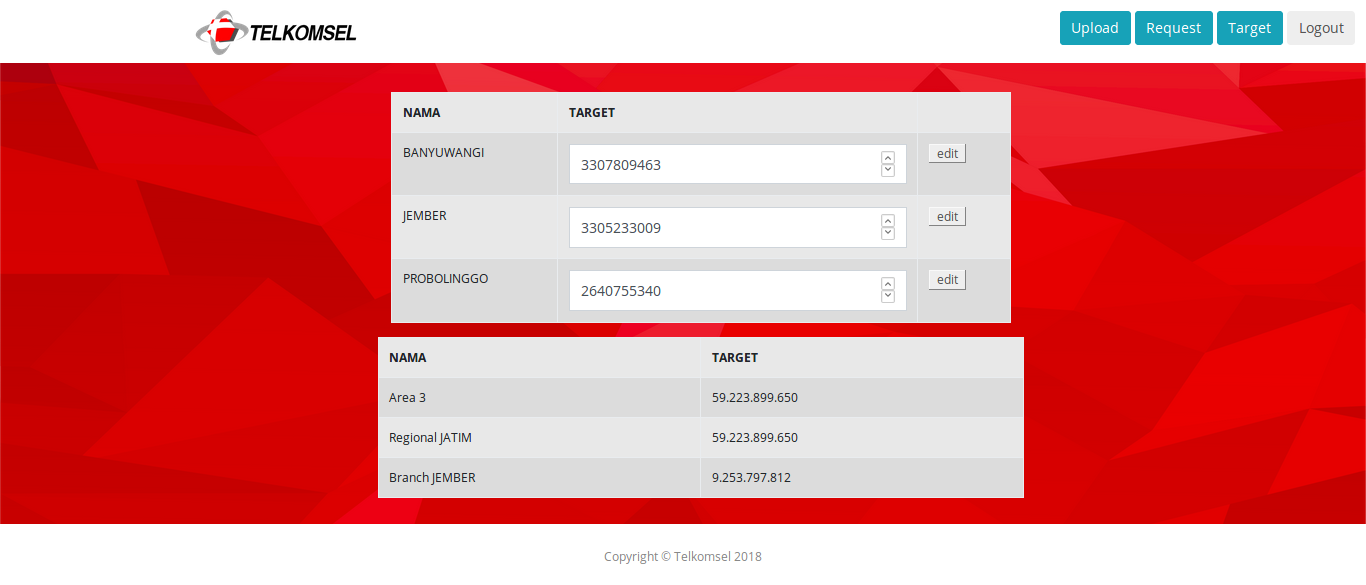
\includegraphics[width=10cm,height=5cm]{bab6/halamanTarget.png}}
\caption{Detail Data Target}
\label{figure:lihatTarget}
\end{figure}

\begin{table}[h!]
	\centering
	\begin{tabular}{|p{4cm}|p{6cm}|}
	\hline
	Kode \textit{Use Case} & UC-002\\ \hline
	Tujuan Pengujian & Menampilkan dan mengubah target pencapaian \textit{revenue}\\ \hline
	Data Masukan & - \\ \hline
	Prosedur Pengujian & 
		\begin{enumerate}
		\item Pengguna \textit{login} sebagai administrator
		\item Pengguna memilih menu target
		\end{enumerate}\\ \hline
	Hasil yang diharapkan & Semua data target pencapaian \textit{revenue} dapat ditampilkan serta dapat diubah pada menu target \\ \hline
	Hasil yang diperoleh & Semua data target pencapaian \textit{revenue} dapat ditampilkan dan diubah \\ \hline
	Kesimpulan & Proses menampilkan dan mengubah data target pencapaian \textit{revenue} berhasil\\ \hline
	Kondisi Akhir & Pengguna mendapatkan semua informasi data target pencapaian serta dapat mengubahnya \textit{revenue}\\ \hline
	\end{tabular}\caption{Skenario Pengujian Menampilkan dan Mengubah Data Target Pencapaian \textit{Revenue}}
	\label{tab:list_target}
\end{table}

\subsection{Pengujian Menampilkan Hasil Pencapaian \textit{Revenue}}
Pengujian ini dilakukan terhadap fungsionalitas menampilkan hasil pencapaian \textit{revenue}. Tabel \ref{tab:list_request} menjelaskan pengujian fungsionalitas ini. Gambar \ref{figure:requestL1}, \ref{figure:requestL3}, dan \ref{figure:requestTop5} adalah hasil fungsionalitas menampilkan hasil pencapaian \textit{revenue}.

\begin{figure}[h!]
	\centerline
	{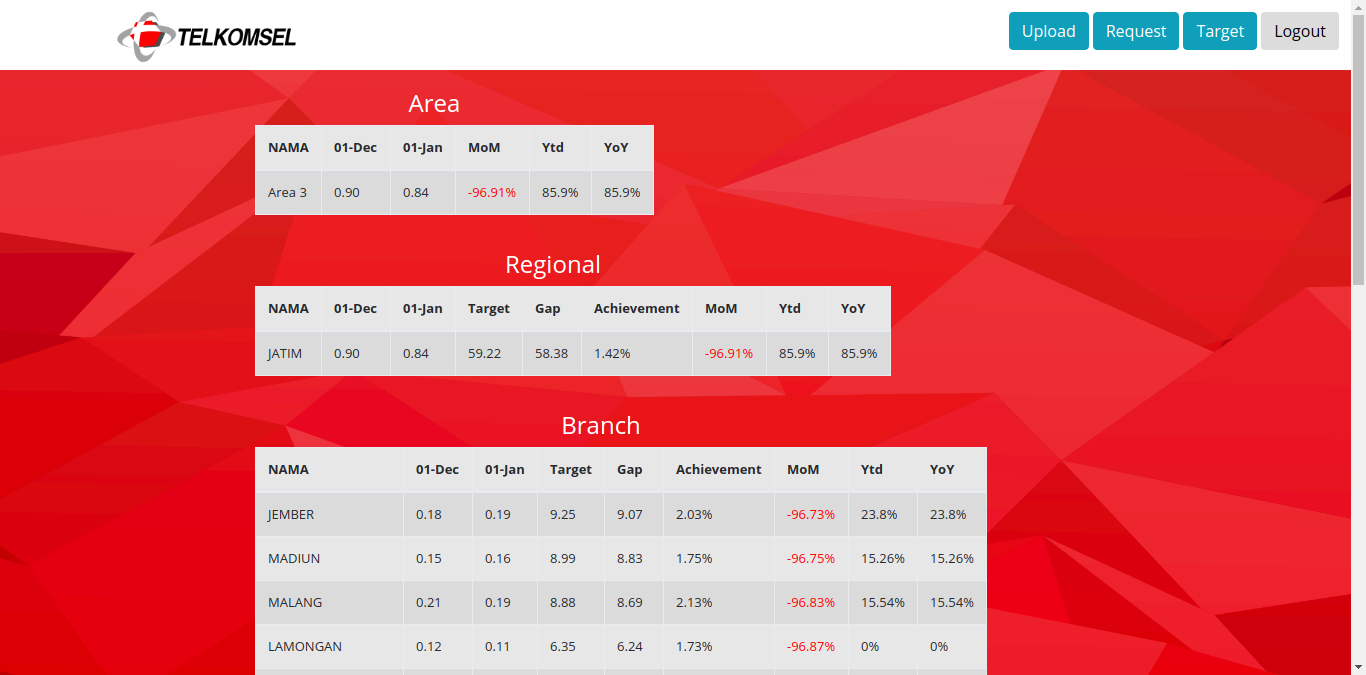
\includegraphics[width=10cm,height=5cm]{bab6/halamanL1.png}}
	\caption{Hasil Pencapaian \textit{Revenue} Berdasarkan L1}
	\label{figure:requestL1}
\end{figure}

\begin{figure}[h!]
	\centerline
	{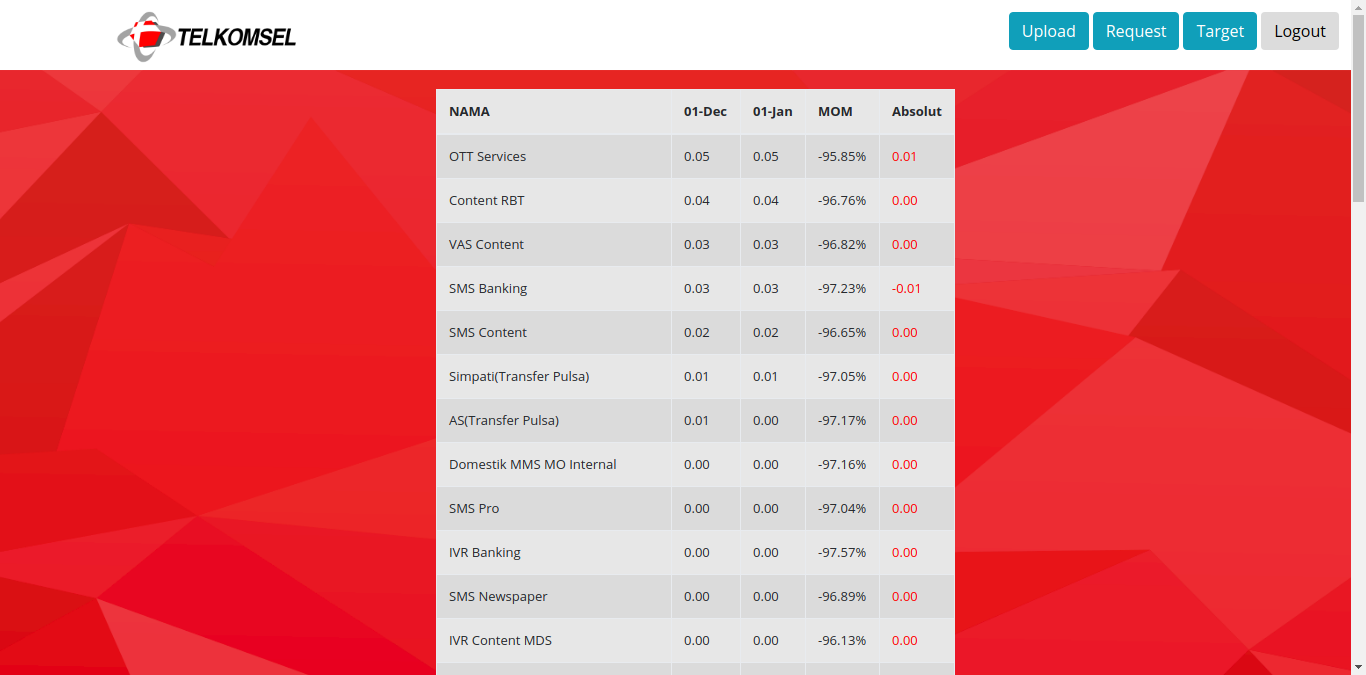
\includegraphics[width=10cm,height=5cm]{bab6/halamanL3.png}}
	\caption{Hasil Pencapaian \textit{Revenue} Berdasarkan L3}
	\label{figure:requestL3}
\end{figure}

\begin{figure}[h!]
	\centerline
	{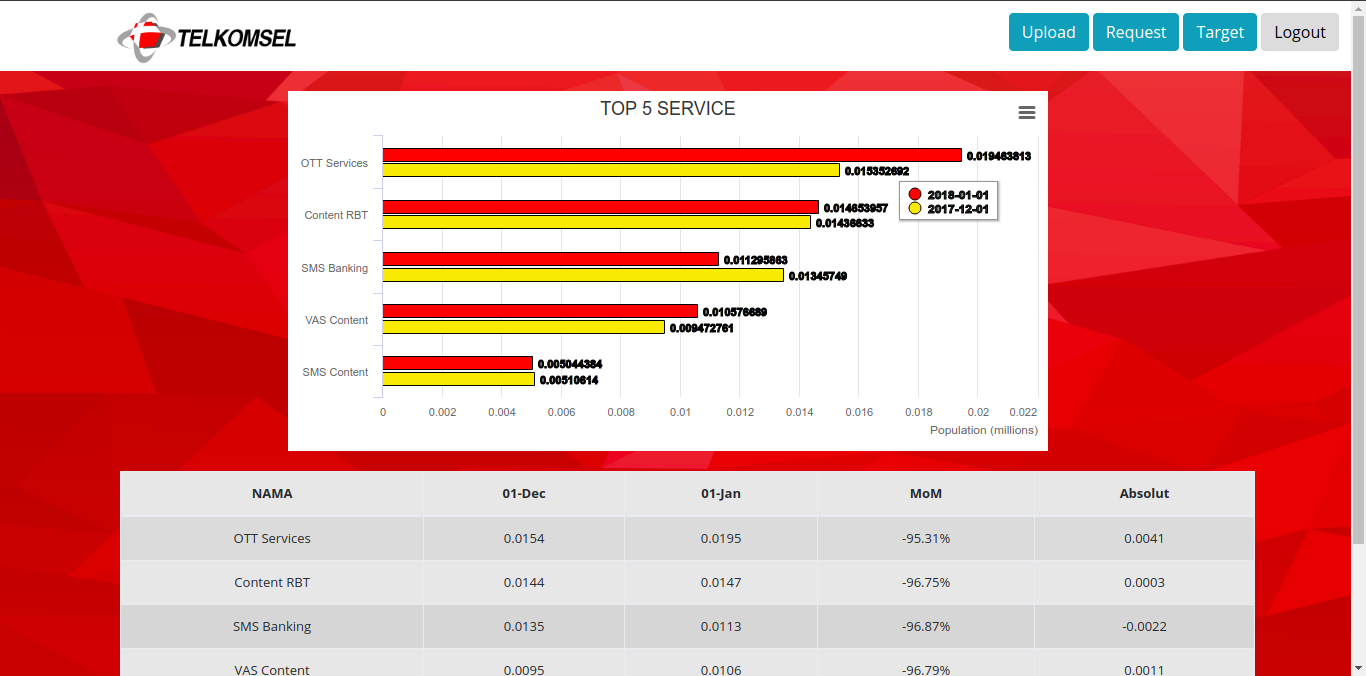
\includegraphics[width=10cm,height=5cm]{bab6/halamanT5.png}}
	\caption{Hasil Pencapaian \textit{Revenue} Berdasarkan Top 5}
	\label{figure:requestTop5}
\end{figure}

\begin{table}[h!]
	\centering
	\begin{tabular}{|p{4cm}|p{6cm}|}
		\hline
		Kode \textit{Use Case} & UC-003\\ \hline
		Tujuan Pengujian & Menampilkan hasil pencapaian \textit{revenue} berdasarkan L1, L3, dan Top 5\\ \hline
		Data Masukan & - \\ \hline
		Prosedur Pengujian & 
		\begin{enumerate}
			\item Pengguna \textit{login} sebagai administrator
			\item Pengguna memilih menu \textit{request}
		\end{enumerate}\\ \hline
		Hasil yang diharapkan & Semua hasil pencapaian \textit{revenue} berdasarkan L1, L3, dan Top5 dapat ditampilkan \\ \hline
		Hasil yang diperoleh & Semua hasil pencapaian \textit{revenue} berdasarkan L1, L3, dan Top5 dapat ditampilkan \\ \hline
		Kesimpulan & Proses menampilkan hasil pencapaian \textit{revenue} berdasarkan L1, L3, dan Top 5 berhasil\\ \hline
		Kondisi Akhir & Pengguna dapat melihat hasil pencapaian \textit{revenue} berdasarkan L1, L3, dan Top 5\\ \hline
	\end{tabular}\caption{Skenario Pengujian Menampilkan Hasil Pencapaian \textit{Revenue}}
	\label{tab:list_request}
\end{table}


\section{Evaluasi Pengujian}
\tab Hasil pengujian dihasilkan dari pengamatan lebih lanjut terhadap perilaku Sistem TPORT terhadap skenario kasus uji coba. Pengujian dilakukan \textit{internal team} untuk mencoba sistem yang telah diterapkan. Tabel \ref{tab:hasil_pengujian} adalah hasil pengujian pada Sistem TPORT.
\begin{table}[h!]
	\centering
	\begin{tabular}{|p{6cm}|p{4cm}|}
	\hline
	\textbf{Tugas} & \textbf{Hasil}\\ \hline
	Sistem mampu menyimpan informasi data pencapaian \textit{revenue} yang di-\textit{upload} oleh pengguna & Terpenuhi\\ \hline
	Sistem mampu menampilkan detail informasi target kepada pengguna & Terpenuhi\\ \hline
	Sistem mampu menangani pengelolaan data target & Terpenuhi\\ \hline
	Sistem mampu menampilkan hasil pencapaian \textit{revenue} & Terpenuhi\\ \hline
	Sistem menampilkan data sesuai dengan opsi yang dipilih oleh pengguna & Terpenuhi\\ \hline
	\end{tabular}\caption{Hasil Pengujian}
		\label{tab:hasil_pengujian}
\end{table}

Dengan hasil pengujian yang telah dilakukan, dapat disimpulkan bahwa keseluruhan Sistem TPORT memenuhi kriteria yang disebutkan pada sub-bab sebelumnya.

\section{Evaluasi Performa}
Tabel \ref{tab:evaluasi_performa} adalah hasil dari uji coba evaluasi performa Sistem TPORT.

\begin{table}
\centering
\begin{tabular}{|p{5cm}|p{2.5cm}|p{2cm}|}
\hline
\textbf{Tugas} & \textbf{Hasil} & \textbf{Waktu}\\ \hline
Membuka halaman login & Terpenuhi & 1 detik\\ \hline
Masuk sebagai pengguna & Terpenuhi & 1 detik\\ \hline
Menampilkan halaman menu & Terpenuhi & 1 detik\\ \hline
Membuka halaman upload & Terpenuhi & 1 detik\\ \hline
Melakukan proses \textit{upload} & Terpenuhi & 10 detik\\ \hline
Membuka halaman \textit{request} & Terpenuhi & 1 detik\\ \hline
Menampilkan hasil \textit{request} & Terpenuhi & 30 detik\\ \hline
Membuka halaman target & Terpenuhi & 1 detik\\ \hline
Menampilkan halaman target & Terpenuhi & 1 detik\\ \hline
\end{tabular}\caption{Hasil Uji Performa}
		\label{tab:evaluasi_performa}
\end{table}

\vspace{4 cm}
\textcolor{white}{..}